% !TeX root = ../../Skript.tex
\cohead{\Large\textbf{Allgemeine Sinus-/Cosinusfunktion}}
\fakesubsection{Allgemeine Sinus- und Cosinusfunktion}
\iftoggle{qrcode}{\setlength{\qrheight}{2.5cm}}{\setlength{\qrheight}{0cm}}%
\newlength{\trigoAllg}%
\setlength{\trigoAllg}{\linewidth-\qrheight}%
\begin{minipage}{\linewidth}
    \adjustbox{valign=t, padding =0ex 0ex 0ex 0ex}{\begin{minipage}{\trigoAllg}
        Die allgemeine Sinusfunktion bzw. Cosinusfunktion sind gegeben durch:

        \[f(x)=\textcolor{red}{a}\sin\left(\textcolor{blue}{b}x\right)+\textcolor{YellowOrange}{d}\qquad g(x)=\textcolor{red}{a}\cos\left(\textcolor{blue}{b}x\right)+\textcolor{YellowOrange}{d}\]
     \end{minipage}}%
    \iftoggle{qrcode}{\adjustbox{valign=t, padding =0ex 0ex 0ex 0ex}{\begin{minipage}{\qrheight}%
                \href{https://www.geogebra.org/m/kuhfc6gm}{
\includegraphics[height=\qrheight]{\trigonometrie/pics/AllgSinCosQR.png}}%
    \end{minipage}}}{}%
\end{minipage}%

\iftoggle{qrcode}{}{\bigskip}%

\begin{itemize}
	\item \(\textcolor{red}{a}\): \textcolor{loes}{Streckfaktor relativ zum Mittelwert in \(y\)-Richtung. Der Betrag von \(a\) gibt die Amplitude an. Für positive \(a\) hat der \(sin\) auf der \(y\)-Achse eine positive Steigung und umgekehrt. Für positive \(a\) hat der \(cos\) auf der \(y\)-Achse einen Hochpunkt, für negative \(a\) einen Tiefpunkt.}

    \bigskip

	\item \(\textcolor{YellowOrange}{d}\): \textcolor{loes}{Verschiebung in \(y\)-Richtung. Da der Mittelwert zuvor bei \(0\) lag, entspricht \(d\) dem Mittelwert.}

    \bigskip

	\item \(\textcolor{blue}{b}\): \textcolor{loes}{Streckfaktor in \(x\)-Richtung. Zwischen dem Streckfaktor und der Periode \(p\) besteht folgender Zusammenhang: \(b\cdot p=2\pi\).}

    \bigskip

\end{itemize}

\bigskip

Beispiel: \(\displaystyle f(x)=\textcolor{red}{2}\sin\left(\textcolor{blue}{0,5}x\right)\textcolor{YellowOrange}{-1}\)

\medskip

\begin{minipage}{\textwidth}
	\includegraphics[width=\textwidth]{\trigonometrie/pics/AllgSin\iftoggle{ausfuellen}{}{_empty}.png}
\end{minipage}

\bigskip

Beispiel: \(\displaystyle g(x)=\textcolor{red}{-0,5}\cos\left(\textcolor{blue}{\pi} x\right)\textcolor{YellowOrange}{+1}\)

\medskip

\begin{minipage}{\textwidth}
	\includegraphics[width=\textwidth]{\trigonometrie/pics/AllgCos\iftoggle{ausfuellen}{}{_empty}.png}
\end{minipage}
\newpage

\begin{Exercise}[title={\raggedright\normalfont Gib jeweils die Amplitude, die Periode und den Mittelwert an. Skizziere dann das Schaubild so, dass mindestens eine Periode zu sehen ist.}, label=allgSinCosA1]

	\begin{enumerate}[label=\alph*)]
		\item \(f_1(x)=-2\sin\left(3x\right)-4\)
		\item \(f_2(x)=1,5\sin\left(4x\right)-2\)
		\item \(f_3(x)=-3\cos\left(0,5x\right)+1\)
		\item \(f_4(x)=\cos\left(\frac{1}{3}x\right)\)
		\item \(f_5(x)=-\sin\left(\frac{1}{2}x\right)-1\)
		\item \(f_6(x)=3\sin\left(\frac{2}{3}x\right)+3\)
		\item \(f_7(x)=4\cos\left(\frac{3}{4}x\right)+2\)
		\item \(f_8(x)=2,5\sin\left(\pi x\right)-1\)
		\item \(f_9(x)=-\cos\left(\frac{\pi}{2}x\right)+2\)
		\item \(f_{10}(x)=-4\sin\left(2\pi x\right)-1\)
		\item \(f_{11}(x)=-2,5\cos\left(4\pi x\right)+3,5\)
		\item \(f_{12}(x)=3\cos\left(1,5x\right)+2\)
		\item \(f_{13}(x)=0,5\sin\left(0,5\pi x\right)+1,5\)
		\item \(f_{14}(x)=-5\sin\left(4\pi x\right)-3\)
		\item \(f_{15}(x)=3\cos\left(x\right)+2\)
		\item \(f_{16}(x)=-2\sin\left(2x\right)\)
		\item \(f_{17}(x)=2,5\sin\left(2x\right)-3,5\)
		\item \(f_{18}(x)=3,5\cos\left(\frac{2}{3}\pi x\right)+2\)
		\item \(f_{19}(x)=5\cos\left(x\right)-4\)
		\item \(f_{20}(x)=-6\cos\left(2\pi x\right)+10\)
	\end{enumerate}
\end{Exercise}
\newpage
%%%%%%%%%%%%%%%%%%%%%%%%%%%%%%%%%%%%%%%%%%%%%%%%%%%%%%%%%%%%%%%%%%%%%%%%%%%%%%%%%%%%%%%%%%%%%%%%%%%%%%%%%%%%%%%%%%%%%%%%
\begin{Exercise}[title={\raggedright\normalfont Stelle jeweils die Funktionsgleichung vom Typ \(a\cdot \sin\left(bx\right)+d\) oder \(a\cdot \cos\left(bx\right)+d\) auf.}, label=allgSinCosA2]

	\begin{minipage}{\textwidth}
		\begin{minipage}{0.5\textwidth}
			\begin{enumerate}[label=\alph*)]
				\item \adjustbox{valign=t}{\begin{minipage}{.9\textwidth-5pt}
					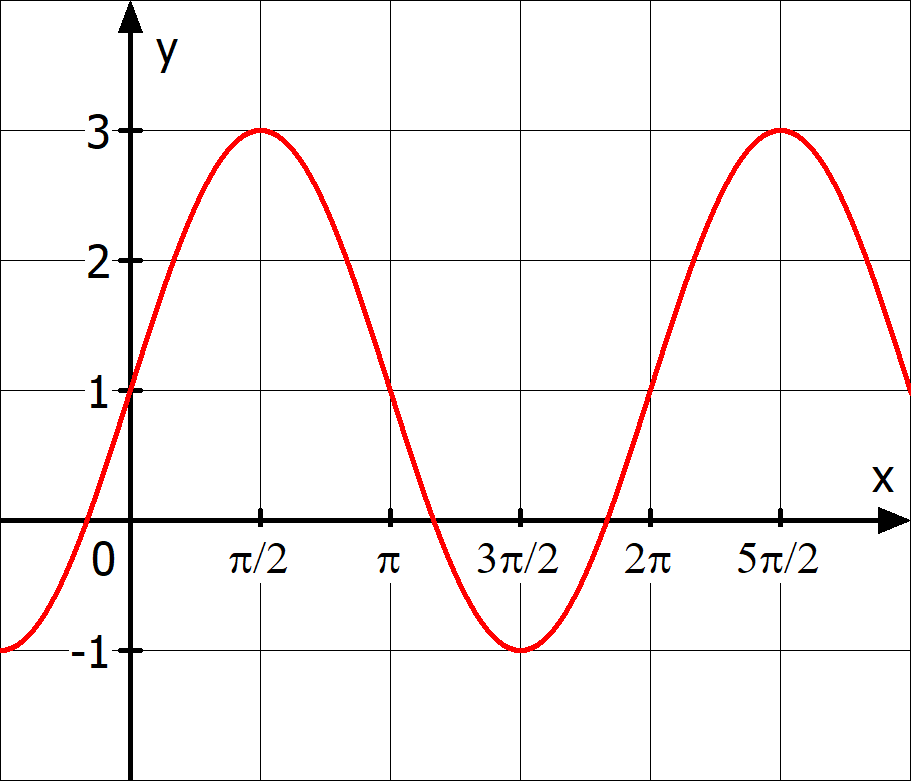
\includegraphics[width=.75\textwidth]{\trigonometrie/pics/AllgSinA2_1.png}
				\end{minipage}}%

                \bigskip

				\item \adjustbox{valign=t}{\begin{minipage}{.9\textwidth-5pt}
					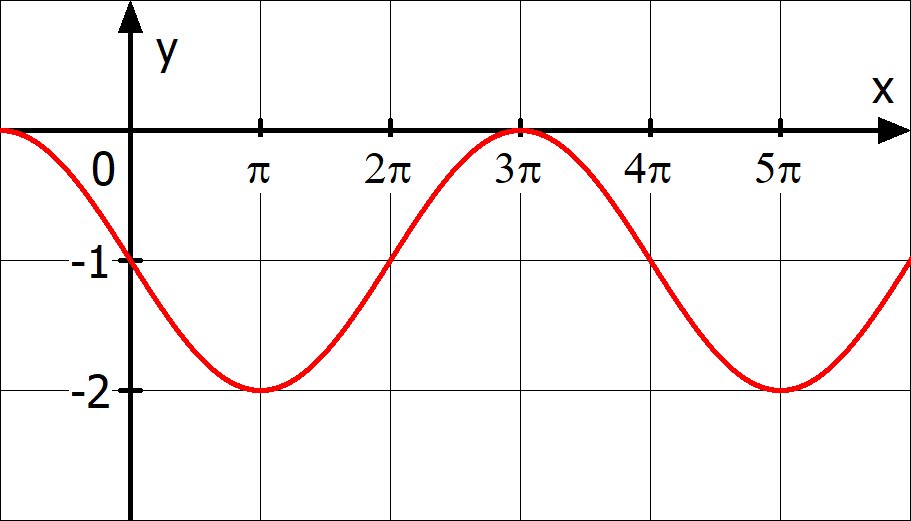
\includegraphics[width=.75\textwidth]{\trigonometrie/pics/AllgSinA2_2.png}
				\end{minipage}}%

                \bigskip

				\item \adjustbox{valign=t}{\begin{minipage}{.9\textwidth-5pt}
					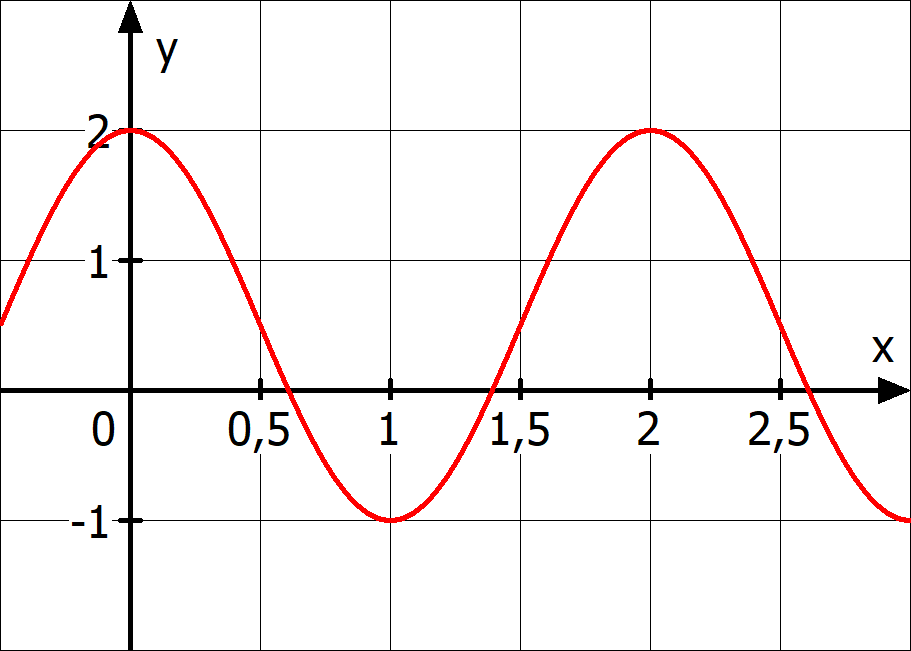
\includegraphics[width=.75\textwidth]{\trigonometrie/pics/AllgSinA2_3.png}
				\end{minipage}}%

                \bigskip

				\item \adjustbox{valign=t}{\begin{minipage}{.9\textwidth-5pt}
					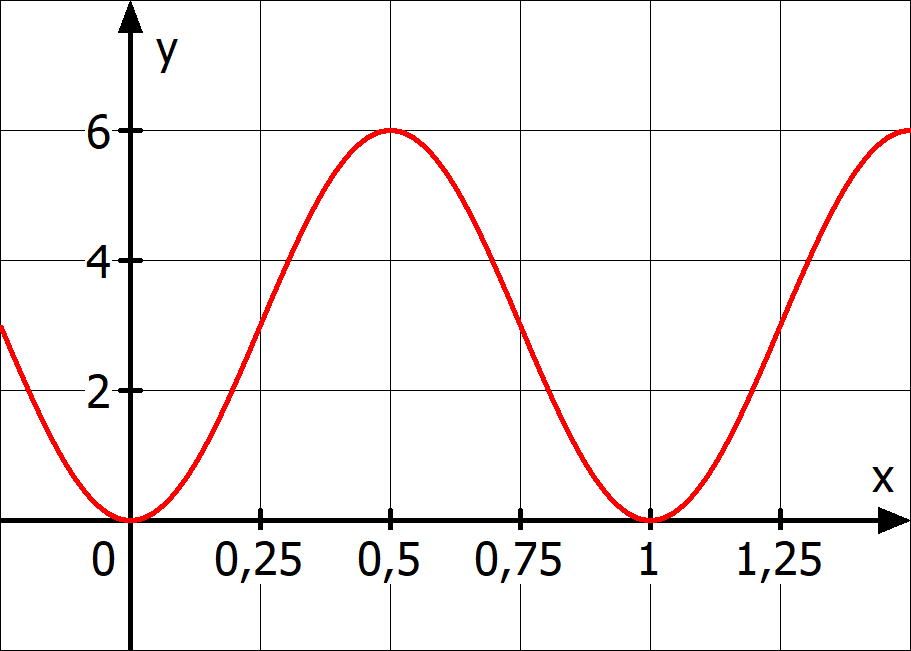
\includegraphics[width=.75\textwidth]{\trigonometrie/pics/AllgSinA2_4.png}
				\end{minipage}}%

                \bigskip

				\item \adjustbox{valign=t}{\begin{minipage}{.9\textwidth-5pt}
					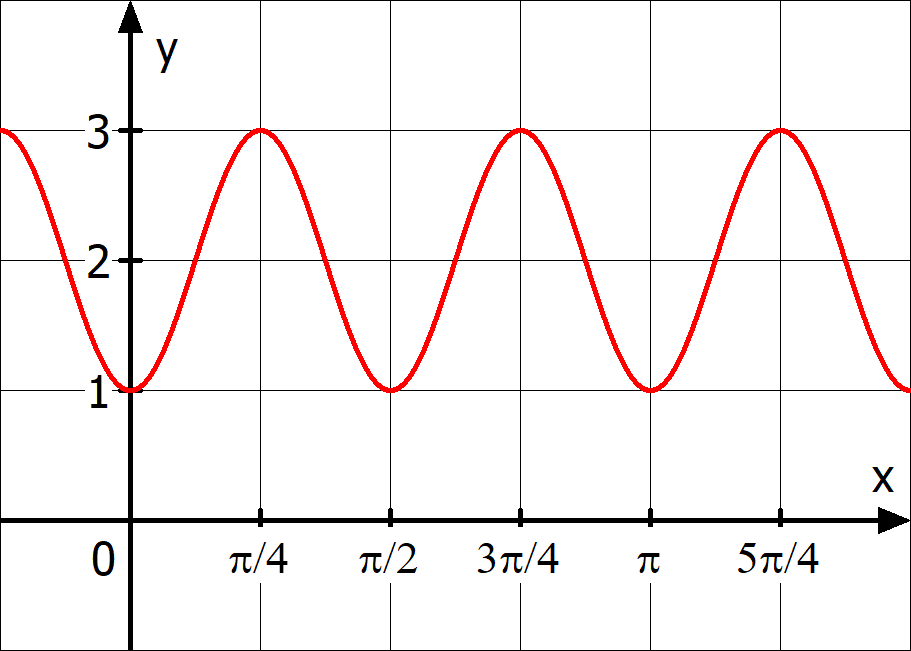
\includegraphics[width=.75\textwidth]{\trigonometrie/pics/AllgSinA2_5.png}
				\end{minipage}}%
			\end{enumerate}
		\end{minipage}%
		\begin{minipage}{0.5\textwidth}
			\begin{enumerate}[label=\alph*)]
				\setcounter{enumi}{5}
				\item \adjustbox{valign=t}{\begin{minipage}{.9\textwidth-5pt}
					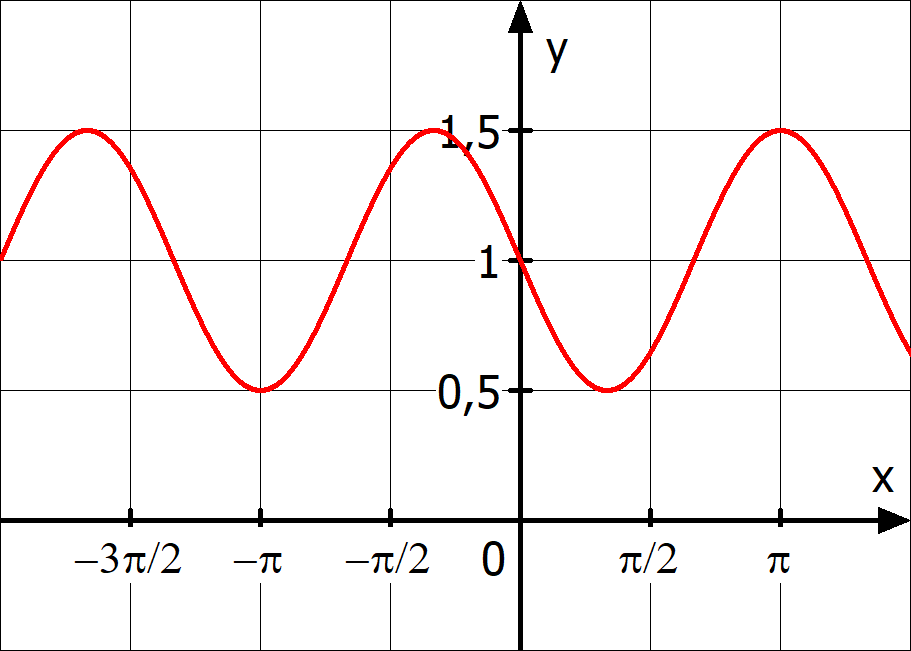
\includegraphics[width=.75\textwidth]{\trigonometrie/pics/AllgSinA2_6.png}
				\end{minipage}}%

                \bigskip

				\item \adjustbox{valign=t}{\begin{minipage}{.9\textwidth-5pt}
					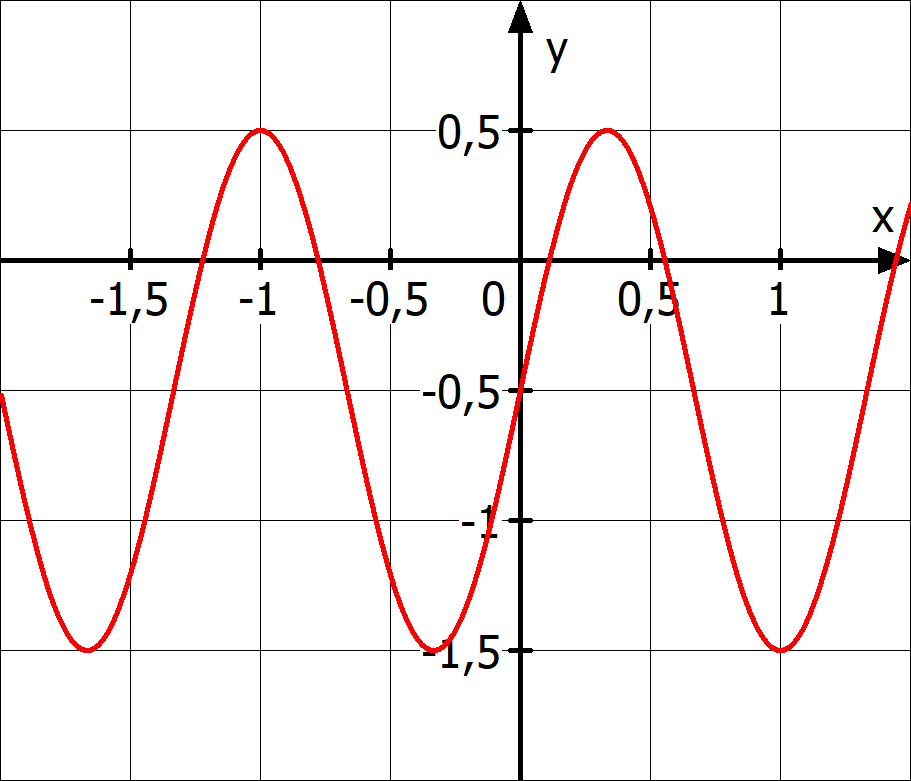
\includegraphics[width=.75\textwidth]{\trigonometrie/pics/AllgSinA2_7.png}
				\end{minipage}}%

                \bigskip

				\item \adjustbox{valign=t}{\begin{minipage}{.9\textwidth-5pt}
					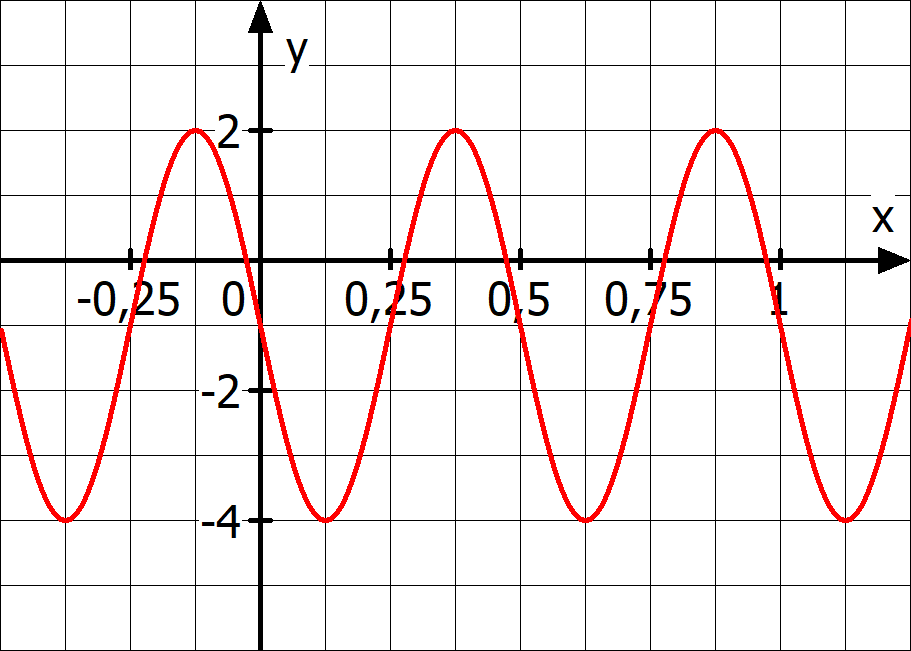
\includegraphics[width=.75\textwidth]{\trigonometrie/pics/AllgSinA2_8.png}
				\end{minipage}}%

                \bigskip

				\item \adjustbox{valign=t}{\begin{minipage}{.9\textwidth-5pt}
					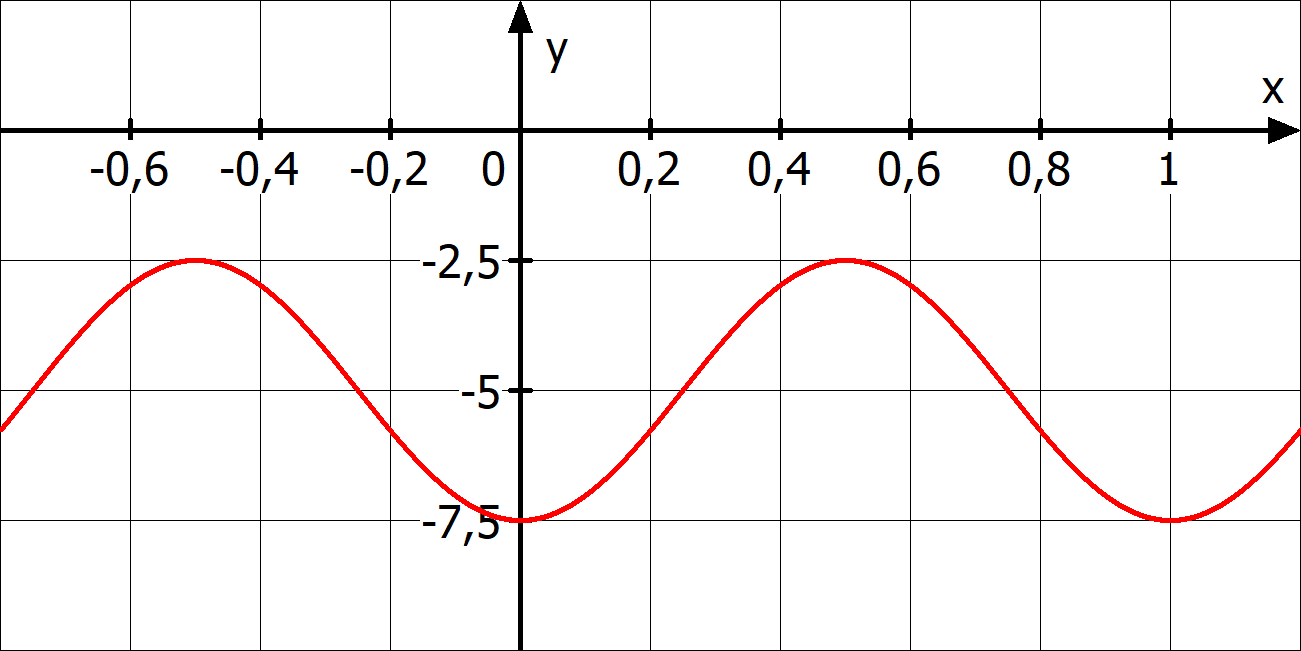
\includegraphics[width=.75\textwidth]{\trigonometrie/pics/AllgSinA2_9.png}
				\end{minipage}}%

                \bigskip

				\item \adjustbox{valign=t}{\begin{minipage}{.9\textwidth-5pt}
					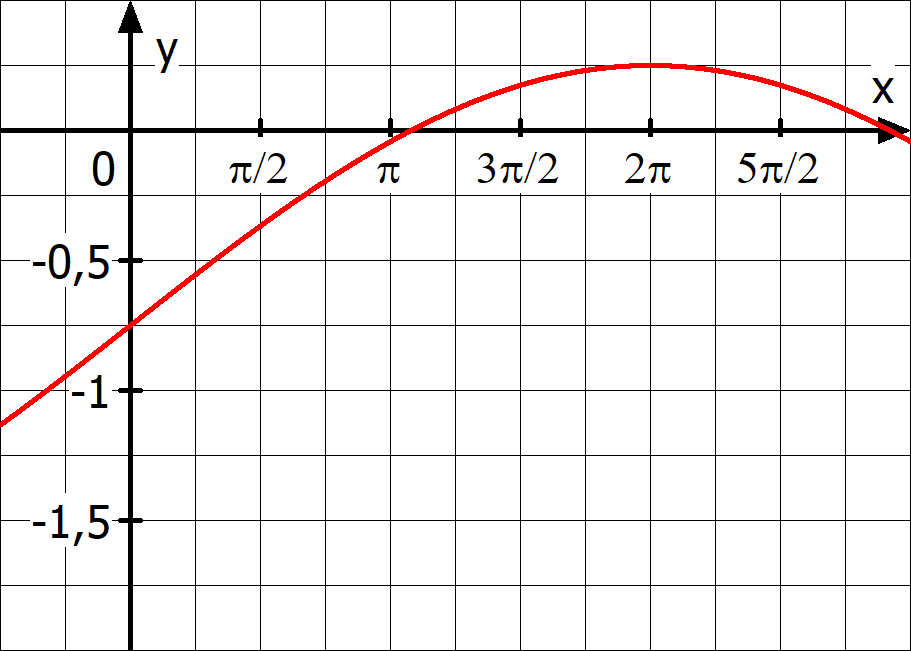
\includegraphics[width=.75\textwidth]{\trigonometrie/pics/AllgSinA2_10.png}
				\end{minipage}}%
			\end{enumerate}
		\end{minipage}%
	\end{minipage}
\end{Exercise}


%%%%%%%%%%%%%%%%%%%%%%%%%%%%%%%%%%%%%%%%%
\begin{Answer}[ref=allgSinCosA1]
	\begin{enumerate}[label=\alph*)]
		\item Amplitude \(a_{1}=2\), Periode \(p_{1}=\frac{2\pi}{3}\), Mittelwert \(d_{1}=-4\)

		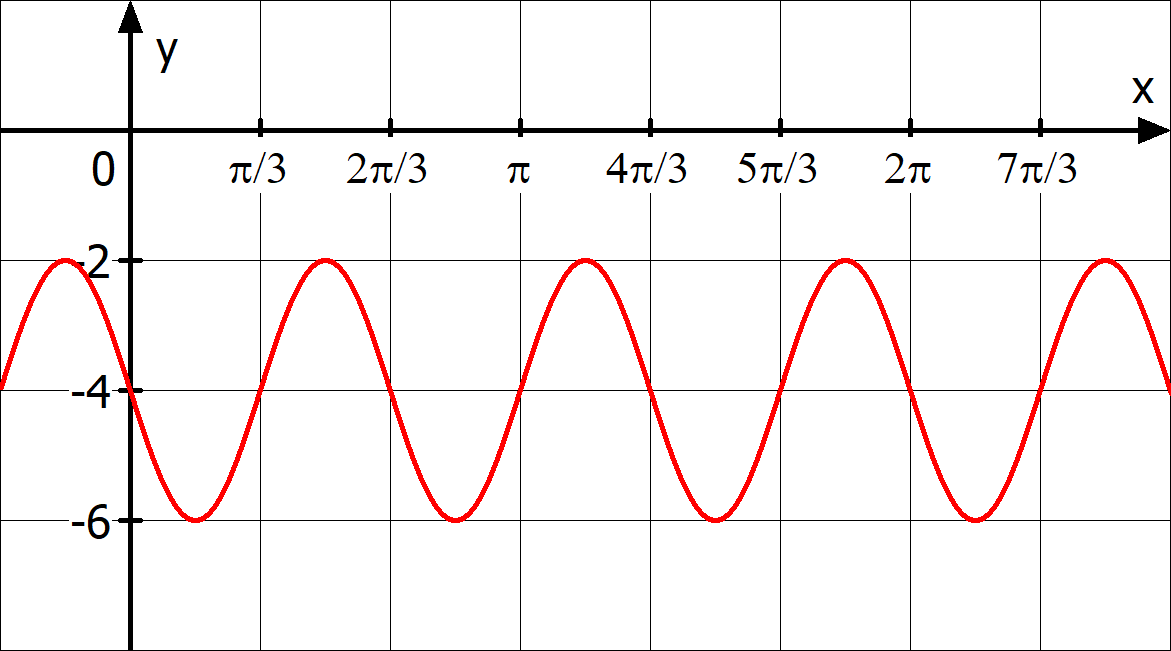
\includegraphics[height=5cm]{\trigonometrie/pics/AllgSinA1_1.png}
		\item Amplitude \(a_{2}=1,5\), Periode \(p_{2}=\frac{\pi}{2}\), Mittelwert \(d_{2}=-2\)

		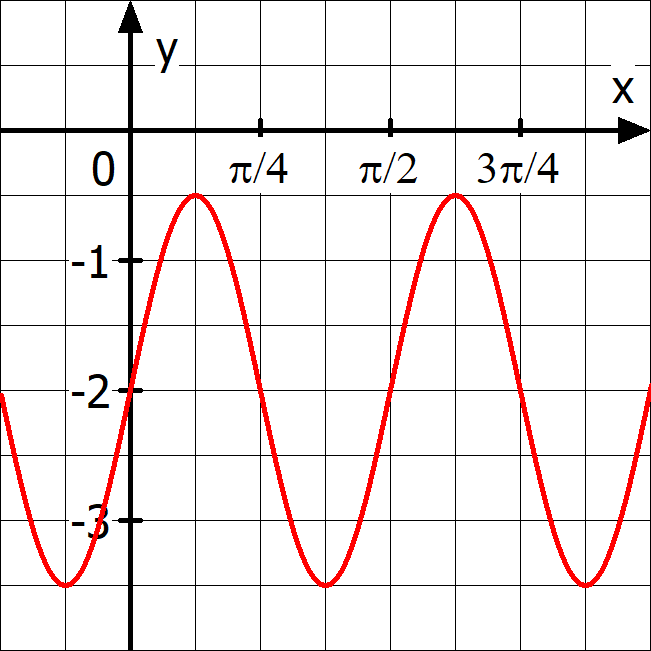
\includegraphics[height=5cm]{\trigonometrie/pics/AllgSinA1_2.png}
		\item Amplitude \(a_{3}=3\), Periode \(p_{3}=4\pi\), Mittelwert \(d_{3}=1\)

		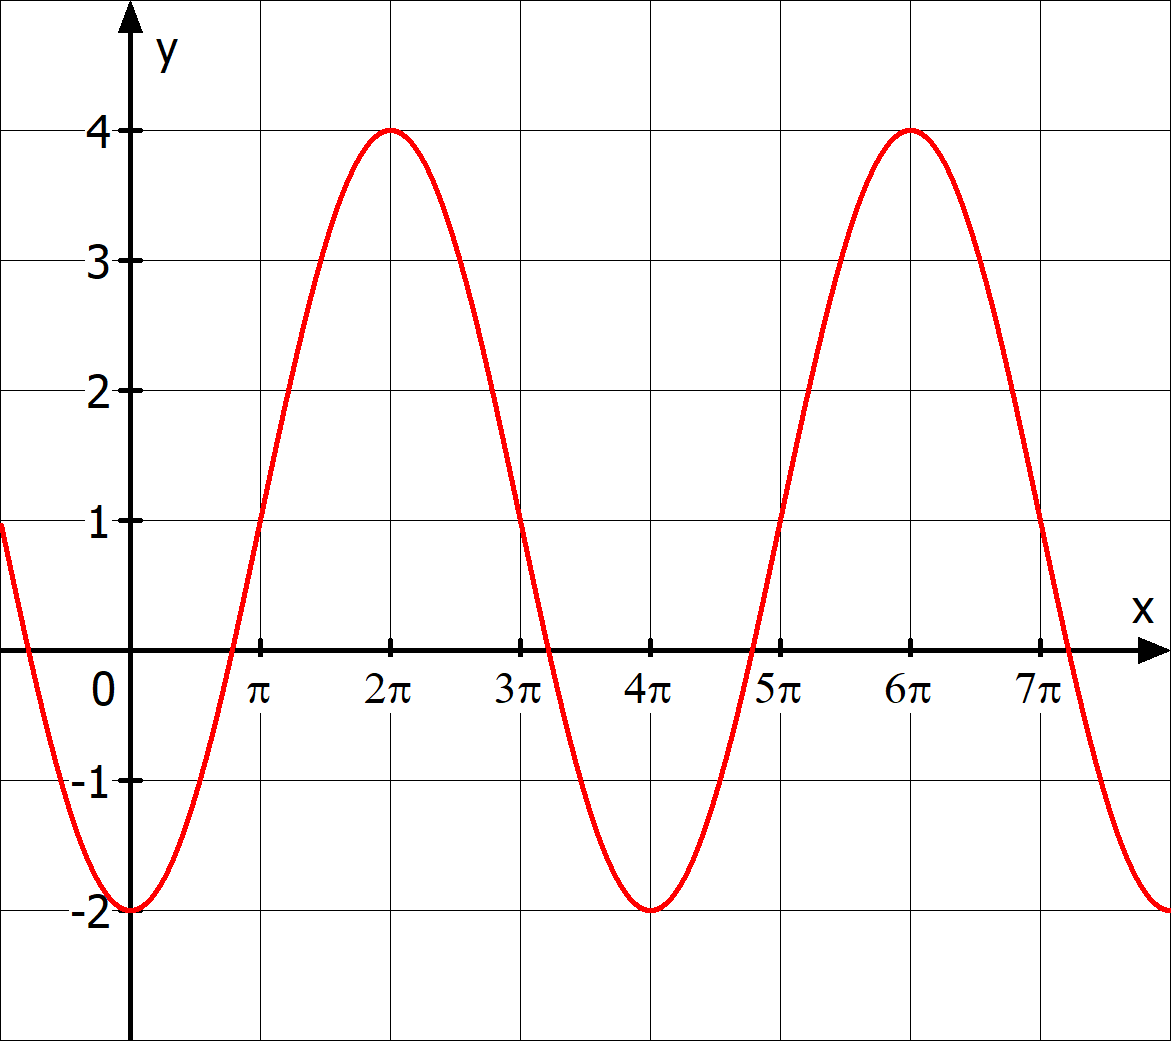
\includegraphics[height=5cm]{\trigonometrie/pics/AllgSinA1_3.png}
		\item Amplitude \(a_{4}=1\), Periode \(p_{4}=6\pi\), Mittelwert \(d_{4}=0\)

		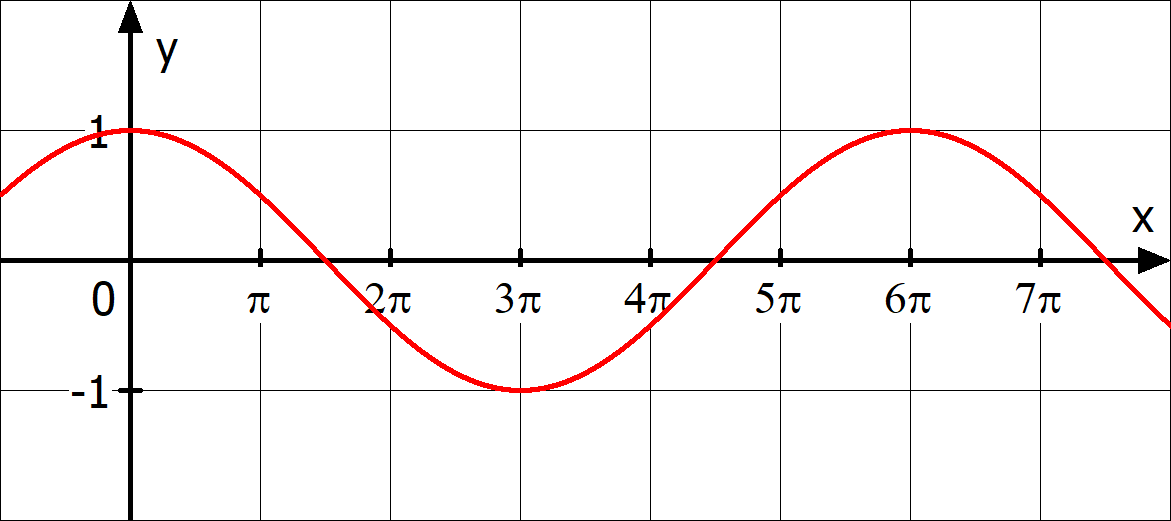
\includegraphics[height=5cm]{\trigonometrie/pics/AllgSinA1_4.png}
        \newpage
		\item Amplitude \(a_{5}=1\), Periode \(p_{5}=4\pi\), Mittelwert \(d_{5}=-1\)

		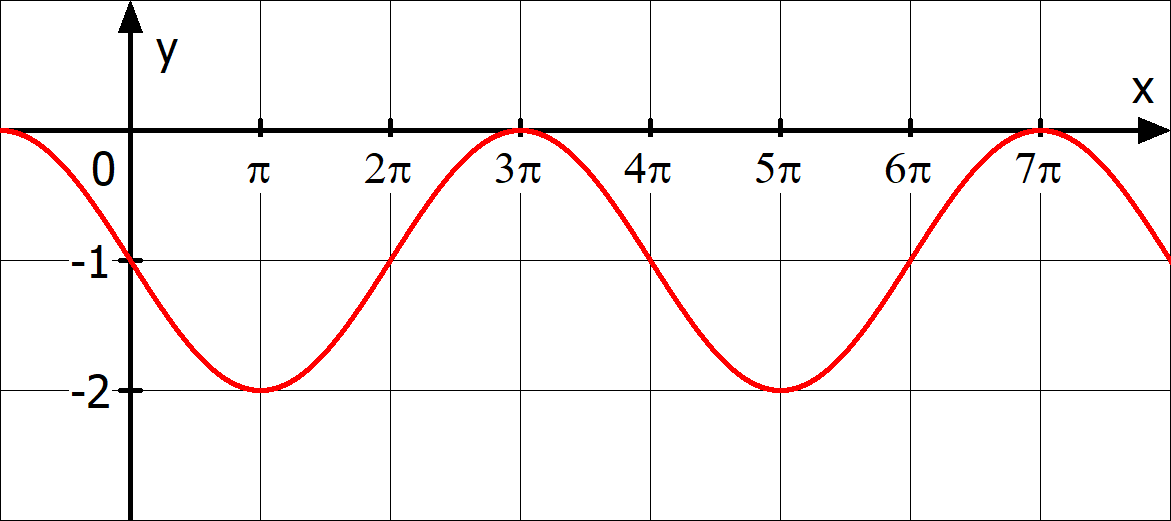
\includegraphics[height=5cm]{\trigonometrie/pics/AllgSinA1_5.png}
		\item Amplitude \(a_{6}=3\), Periode \(p_{6}=3\pi\), Mittelwert \(d_{6}=3\)

		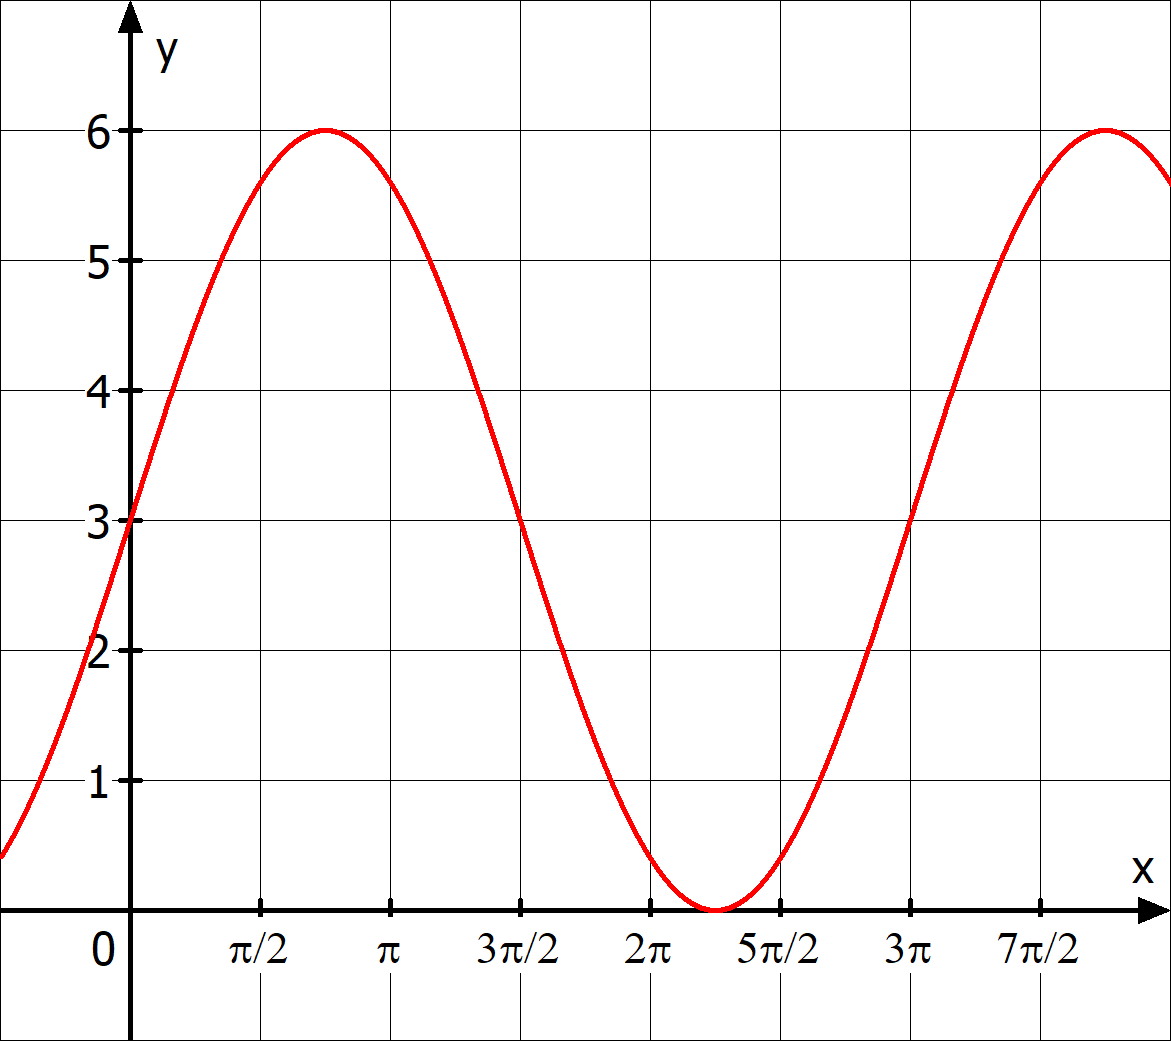
\includegraphics[height=5cm]{\trigonometrie/pics/AllgSinA1_6.png}
		\item Amplitude \(a_{7}=4\), Periode \(p_{7}=\frac{8\pi}{3}\), Mittelwert \(d_{7}=2\)

		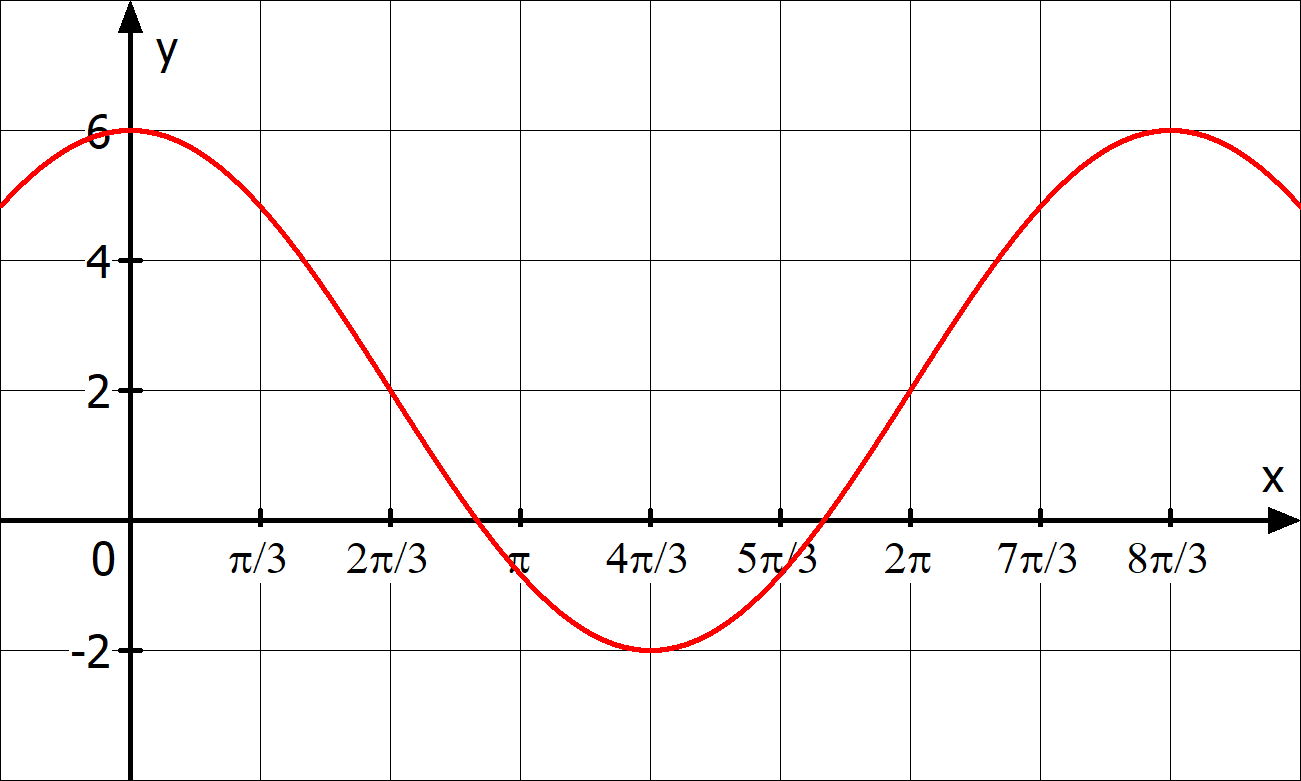
\includegraphics[height=5cm]{\trigonometrie/pics/AllgSinA1_7.png}
		\item Amplitude \(a_{8}=2,5\), Periode \(p_{8}=2\), Mittelwert \(d_{8}=-1\)

		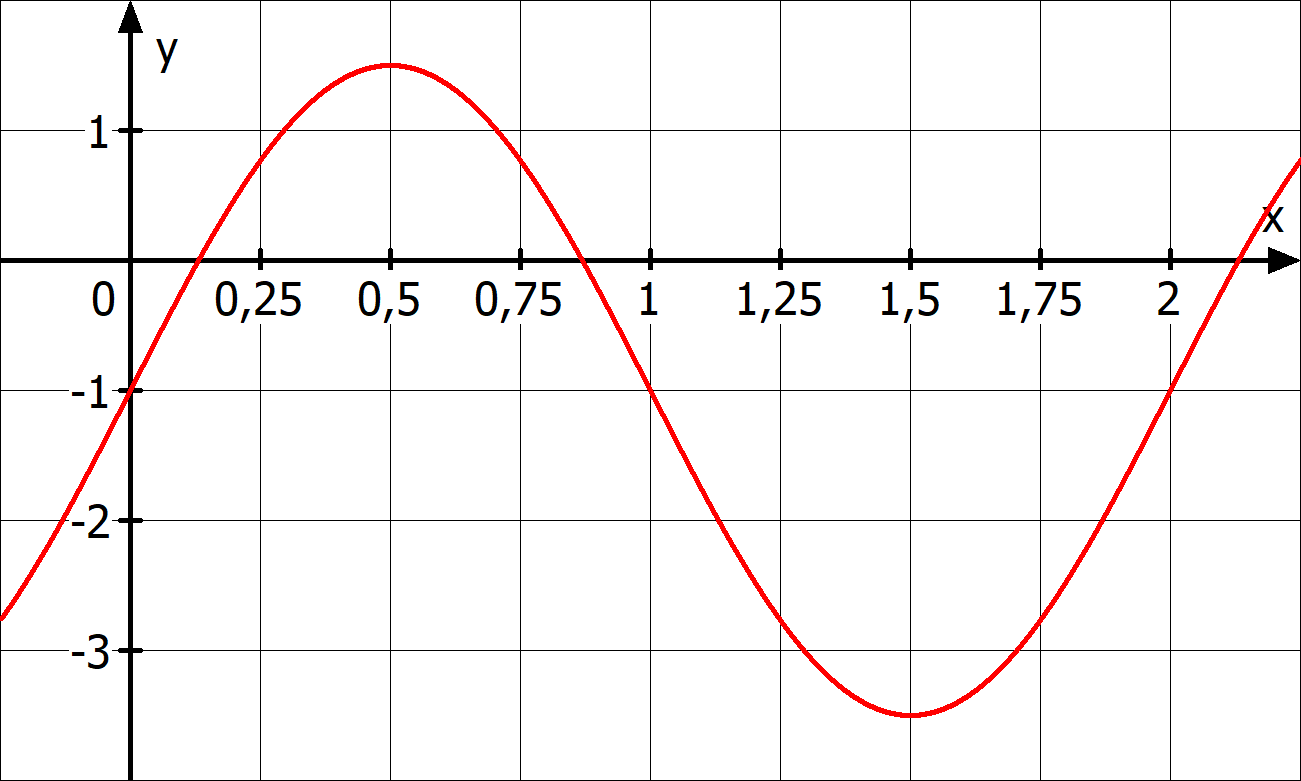
\includegraphics[height=5cm]{\trigonometrie/pics/AllgSinA1_8.png}
        \newpage
		\item Amplitude \(a_{9}=1\), Periode \(p_{9}=4\), Mittelwert \(d_{9}=2\)

		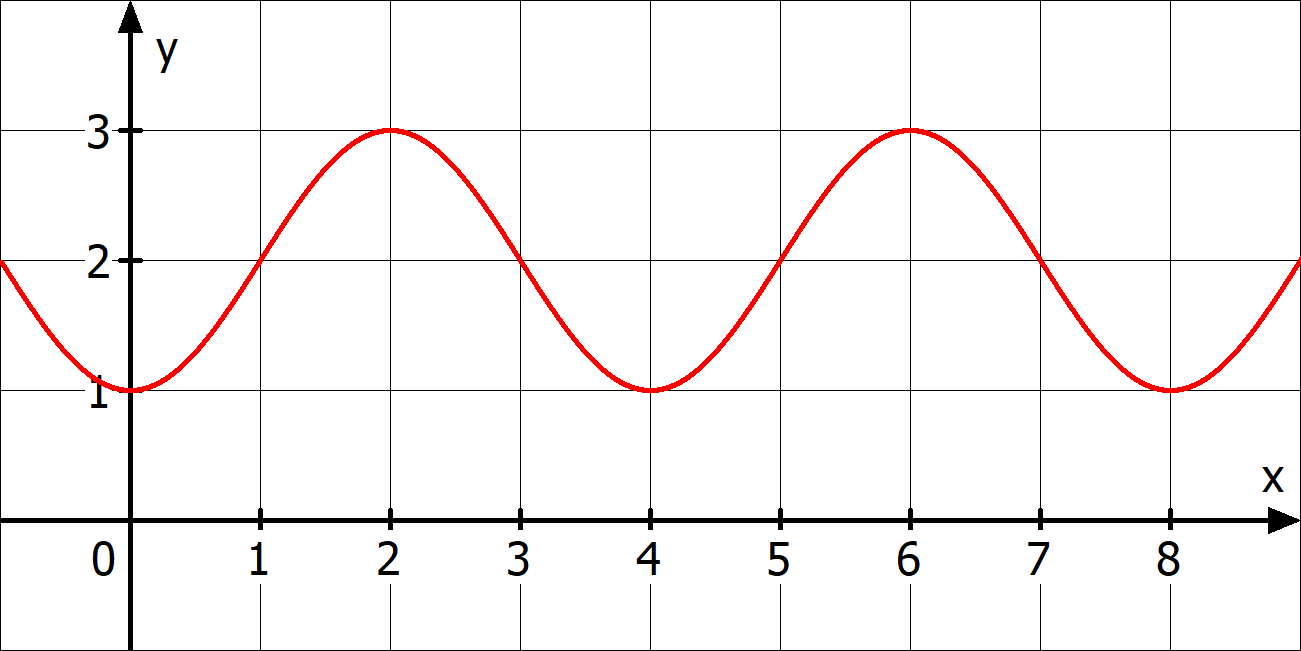
\includegraphics[height=5cm]{\trigonometrie/pics/AllgSinA1_9.png}
		\item Amplitude \(a_{10}=4\), Periode \(p_{10}=1\), Mittelwert \(d_{10}=-1\)

		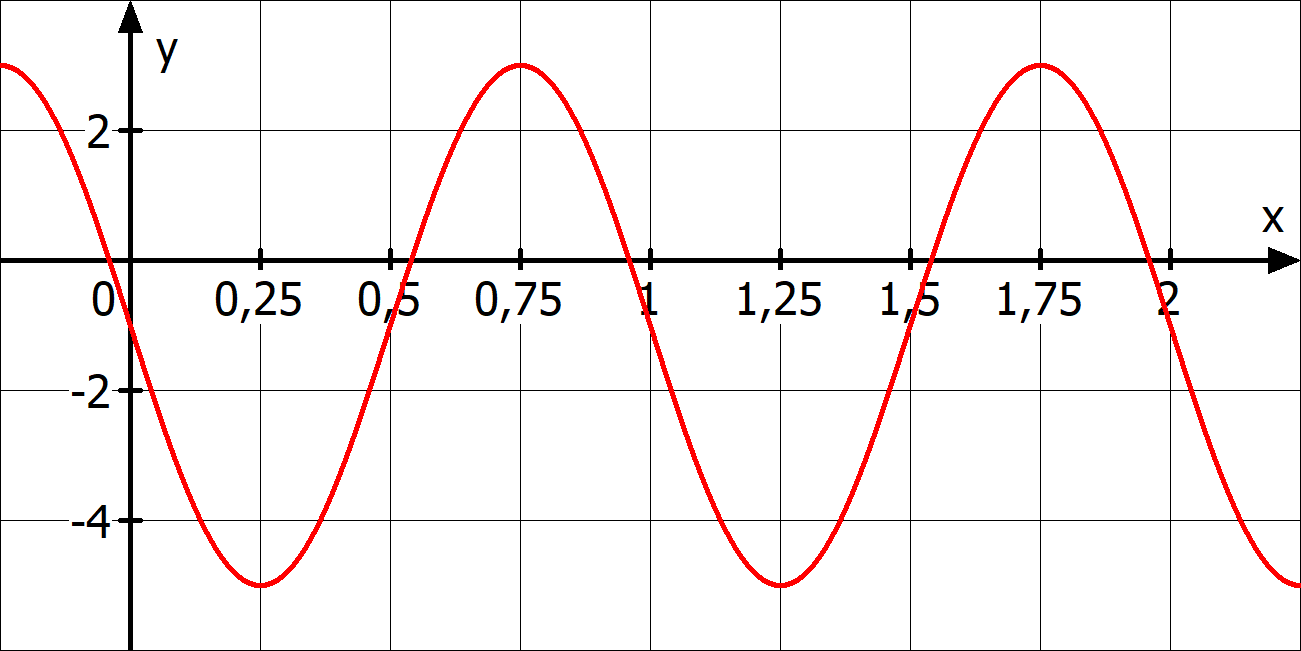
\includegraphics[height=5cm]{\trigonometrie/pics/AllgSinA1_10.png}
		\item Amplitude \(a_{11}=2,5\), Periode \(p_{11}=\frac{1}{2}\), Mittelwert \(d_{11}=3,5\)

		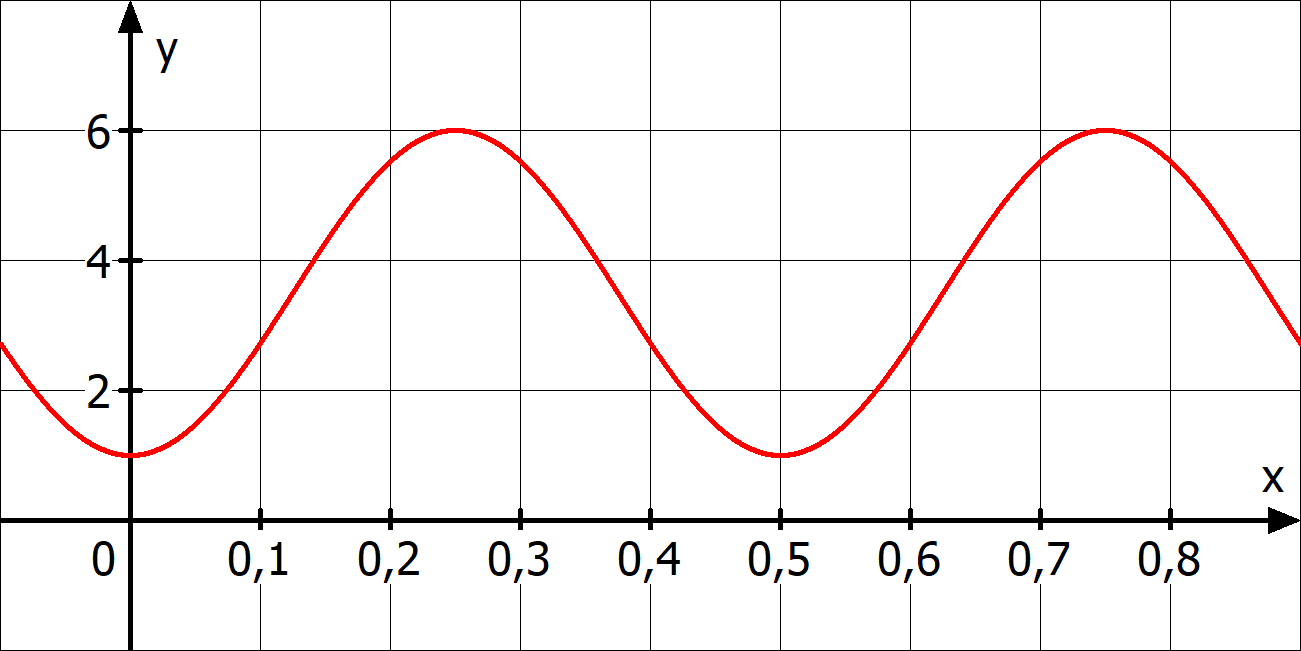
\includegraphics[height=5cm]{\trigonometrie/pics/AllgSinA1_11.png}
		\item Amplitude \(a_{12}=3\), Periode \(p_{12}=\frac{4\pi}{3}\), Mittelwert \(d_{12}=2\)

		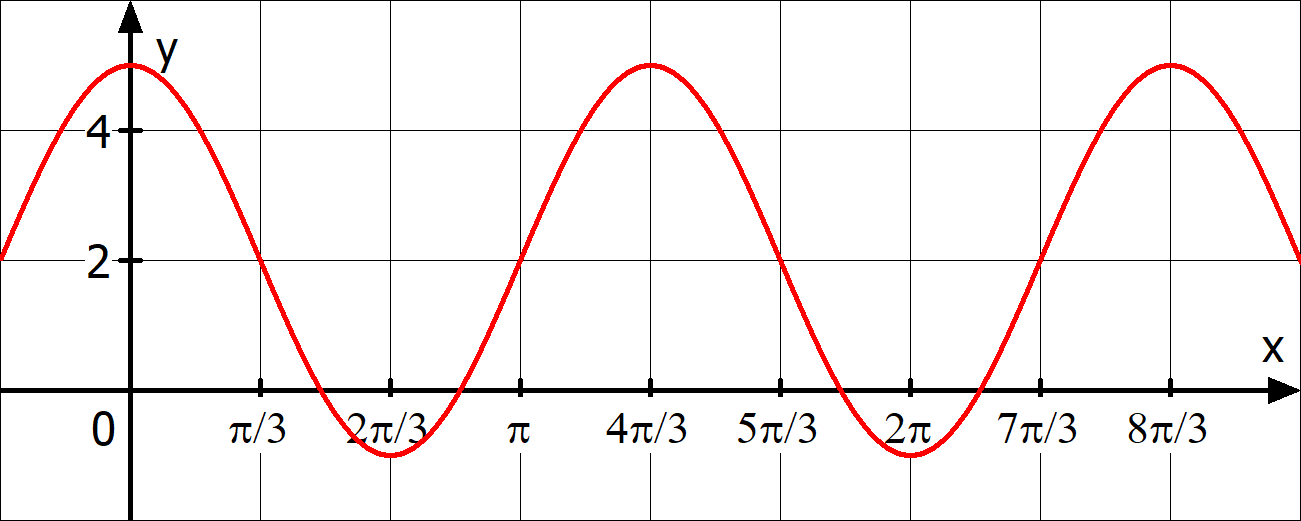
\includegraphics[height=5cm]{\trigonometrie/pics/AllgSinA1_12.png}
        \newpage
		\item Amplitude \(a_{13}=0,5\), Periode \(p_{13}=4\), Mittelwert \(d_{13}=1,5\)

		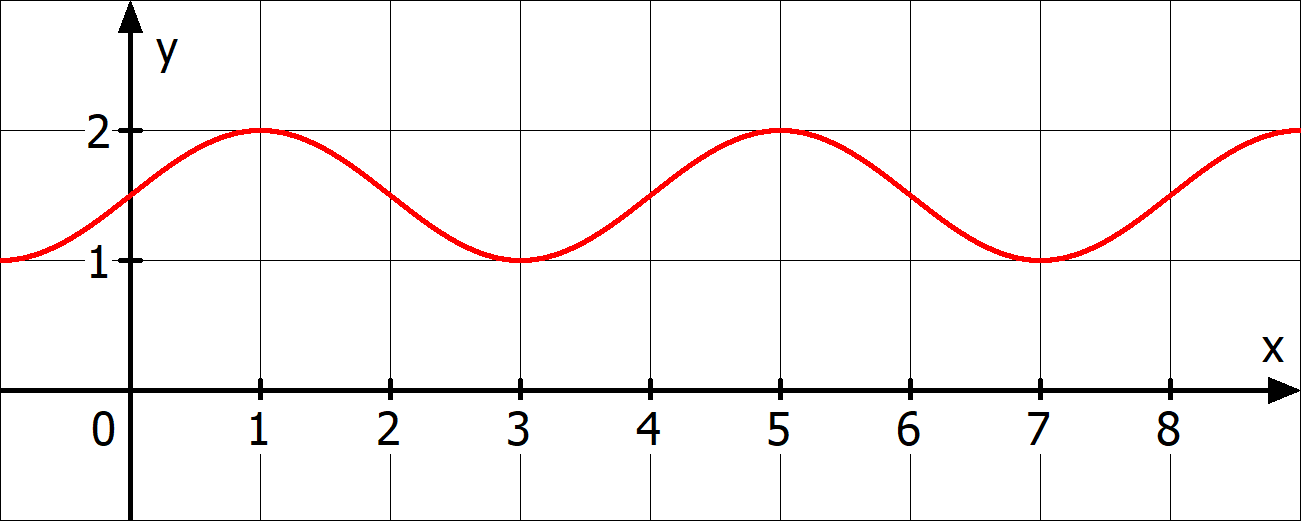
\includegraphics[height=5cm]{\trigonometrie/pics/AllgSinA1_13.png}
		\item Amplitude \(a_{14}=5\), Periode \(p_{14}=0,5\), Mittelwert \(d_{14}=-3\)

		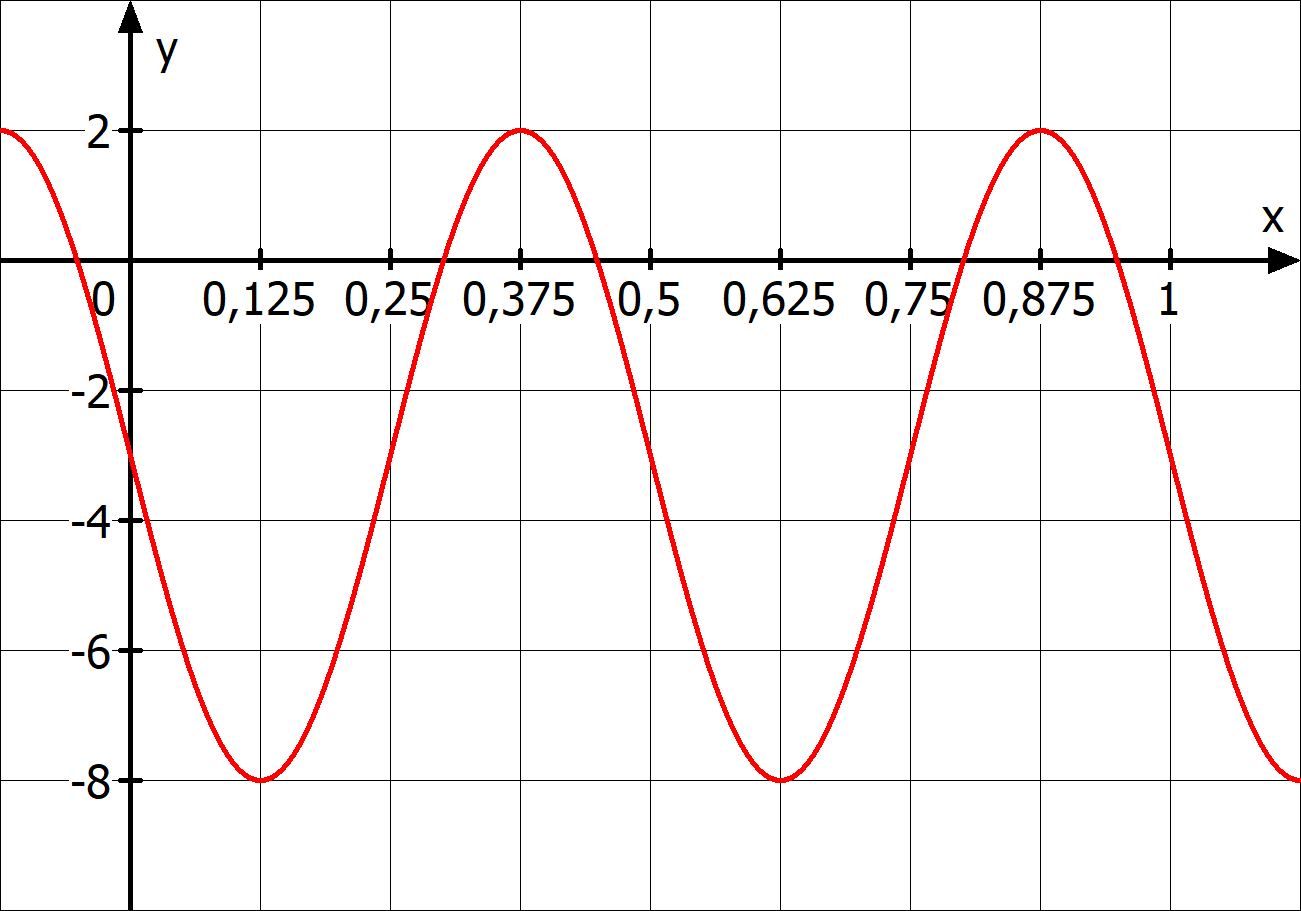
\includegraphics[height=5cm]{\trigonometrie/pics/AllgSinA1_14.png}
		\item Amplitude \(a_{15}=3\), Periode \(p_{15}=2\pi\), Mittelwert \(d_{15}=2\)

		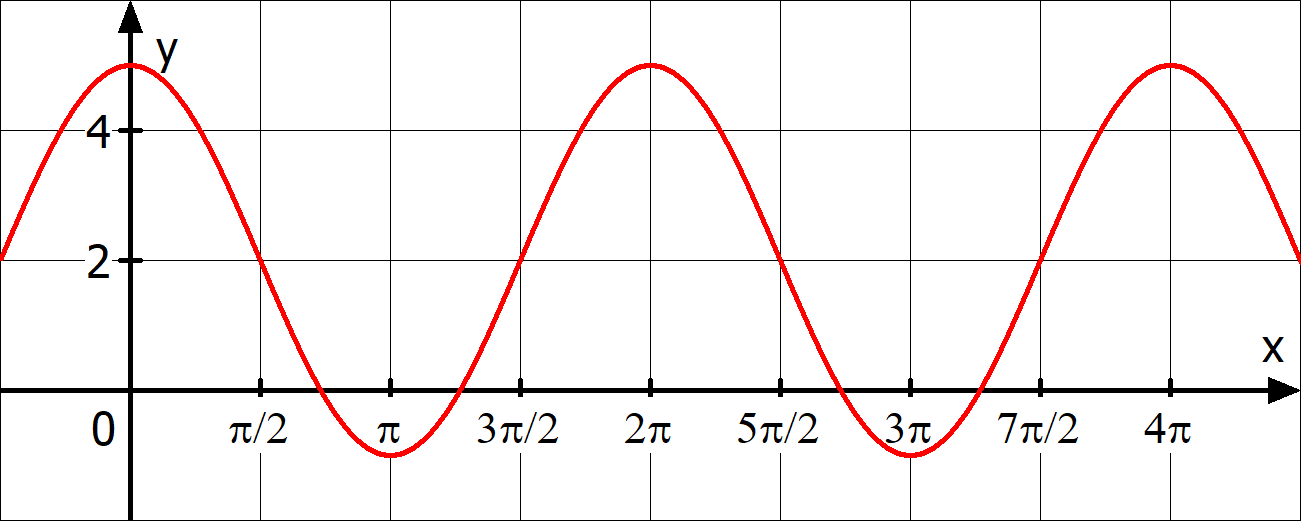
\includegraphics[height=5cm]{\trigonometrie/pics/AllgSinA1_15.png}
		\item Amplitude \(a_{16}=2\), Periode \(p_{16}=\pi\), Mittelwert \(d_{16}=0\)

		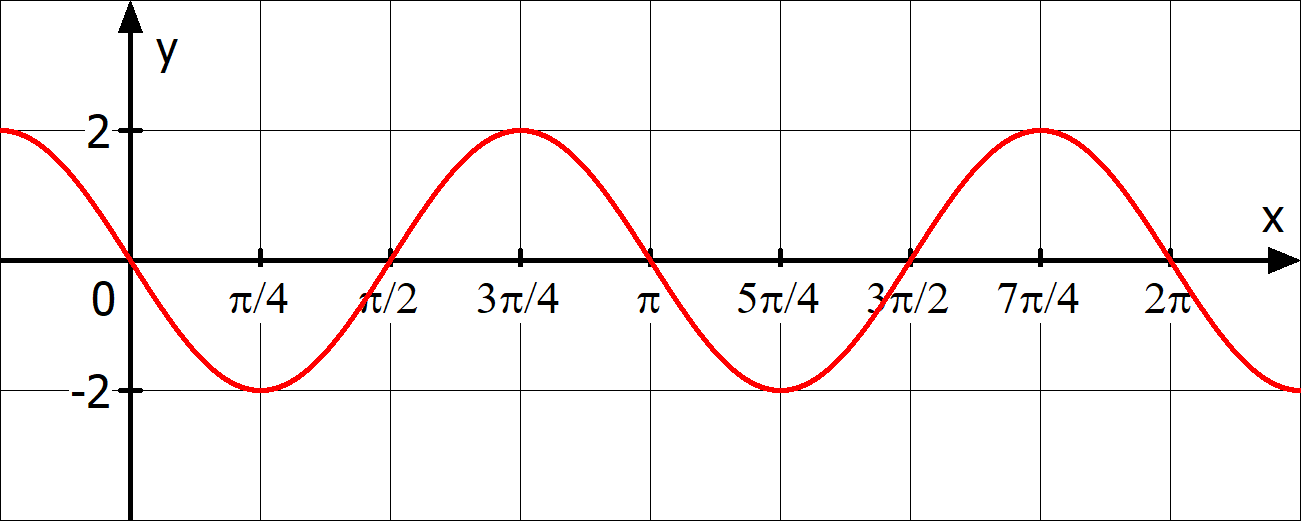
\includegraphics[height=5cm]{\trigonometrie/pics/AllgSinA1_16.png}
        \newpage
		\item Amplitude \(a_{17}=2,5\), Periode \(p_{17}=\pi\), Mittelwert \(d_{17}=-3,5\)

		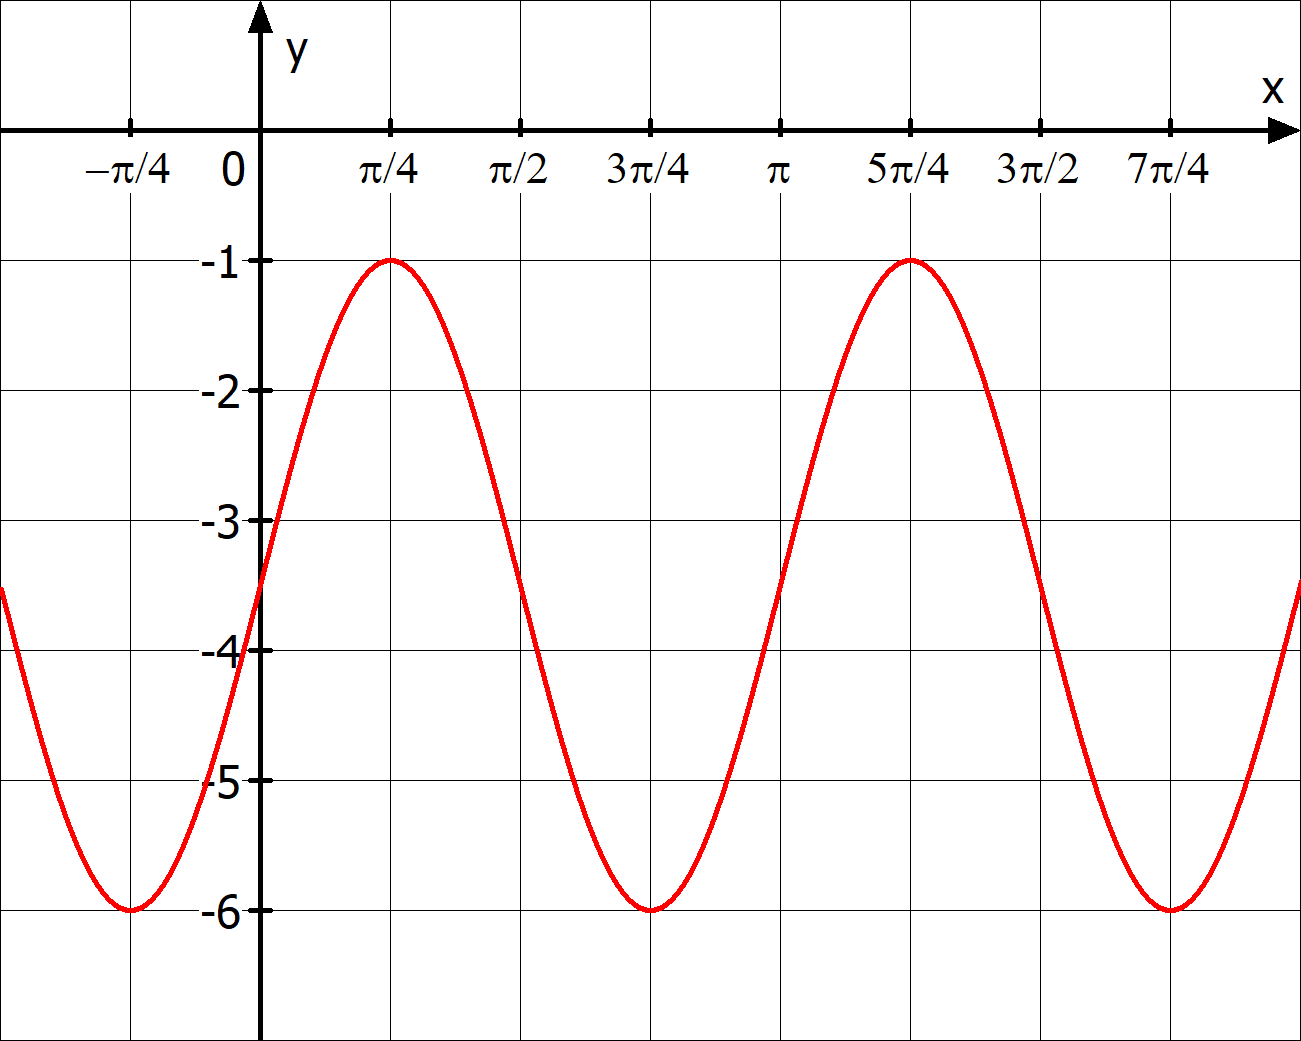
\includegraphics[height=5cm]{\trigonometrie/pics/AllgSinA1_17.png}
		\item Amplitude \(a_{18}=3,5\), Periode \(p_{18}=3\), Mittelwert \(d_{18}=2\)

		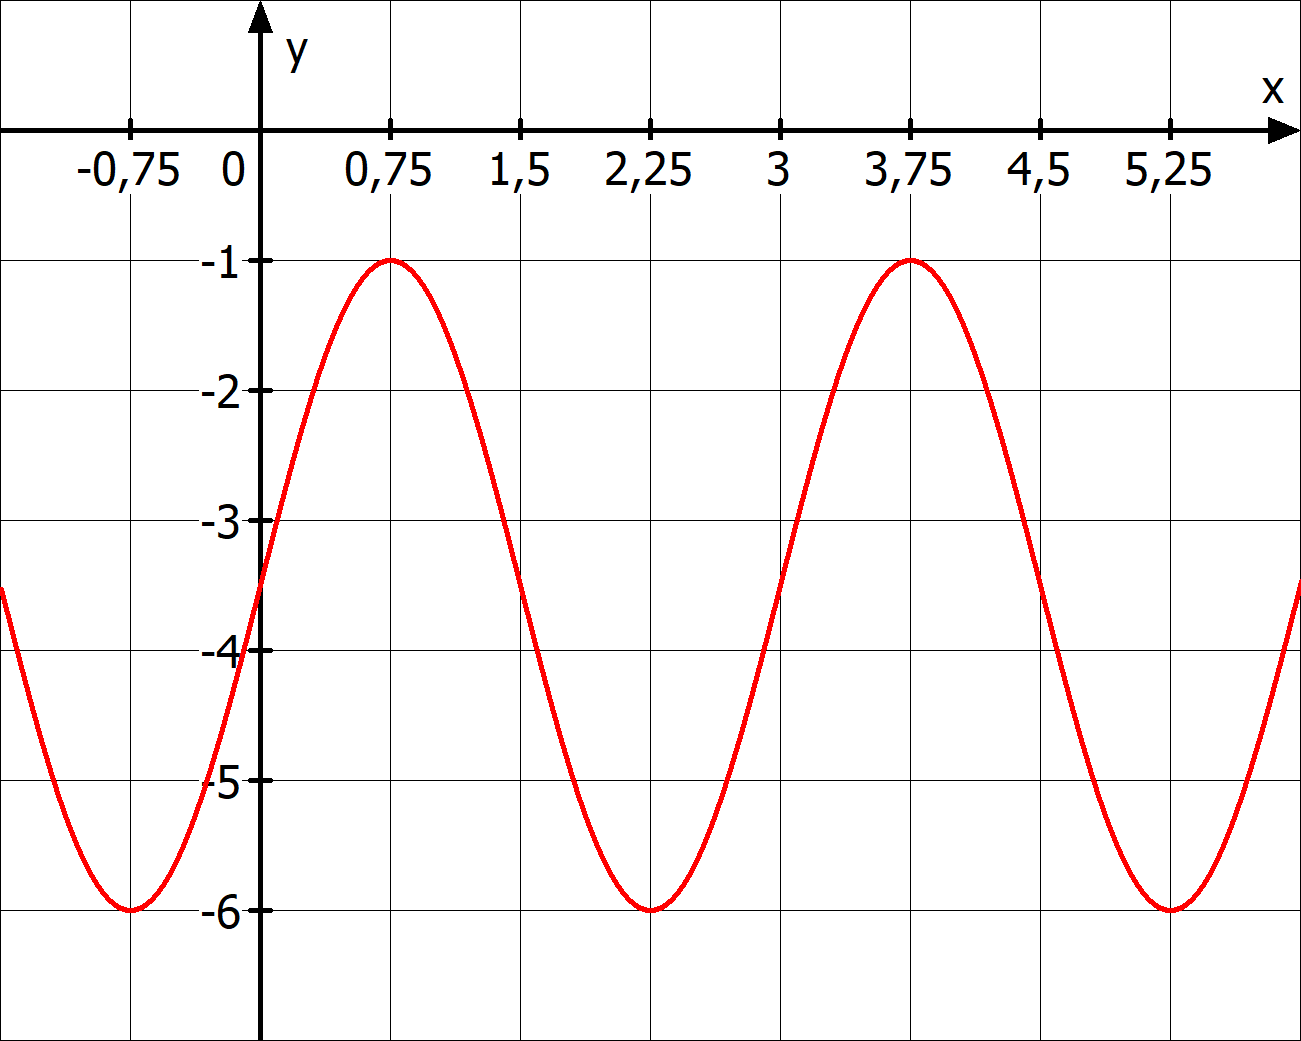
\includegraphics[height=5cm]{\trigonometrie/pics/AllgSinA1_18.png}
		\item Amplitude \(a_{19}=5\), Periode \(p_{19}=2\pi\), Mittelwert \(d_{19}=-4\)

		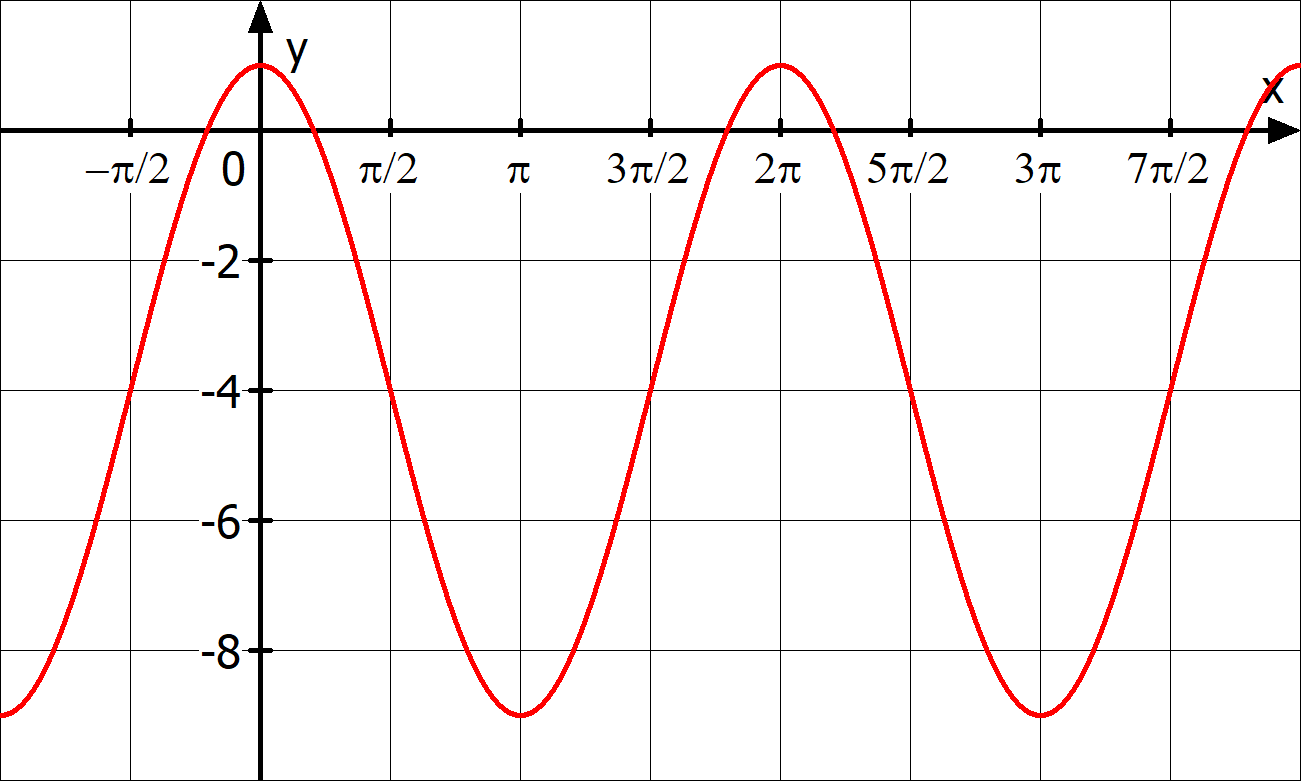
\includegraphics[height=5cm]{\trigonometrie/pics/AllgSinA1_19.png}
		\item Amplitude \(a_{20}=6\), Periode \(p_{20}=1\), Mittelwert \(d_{20}=10\)

		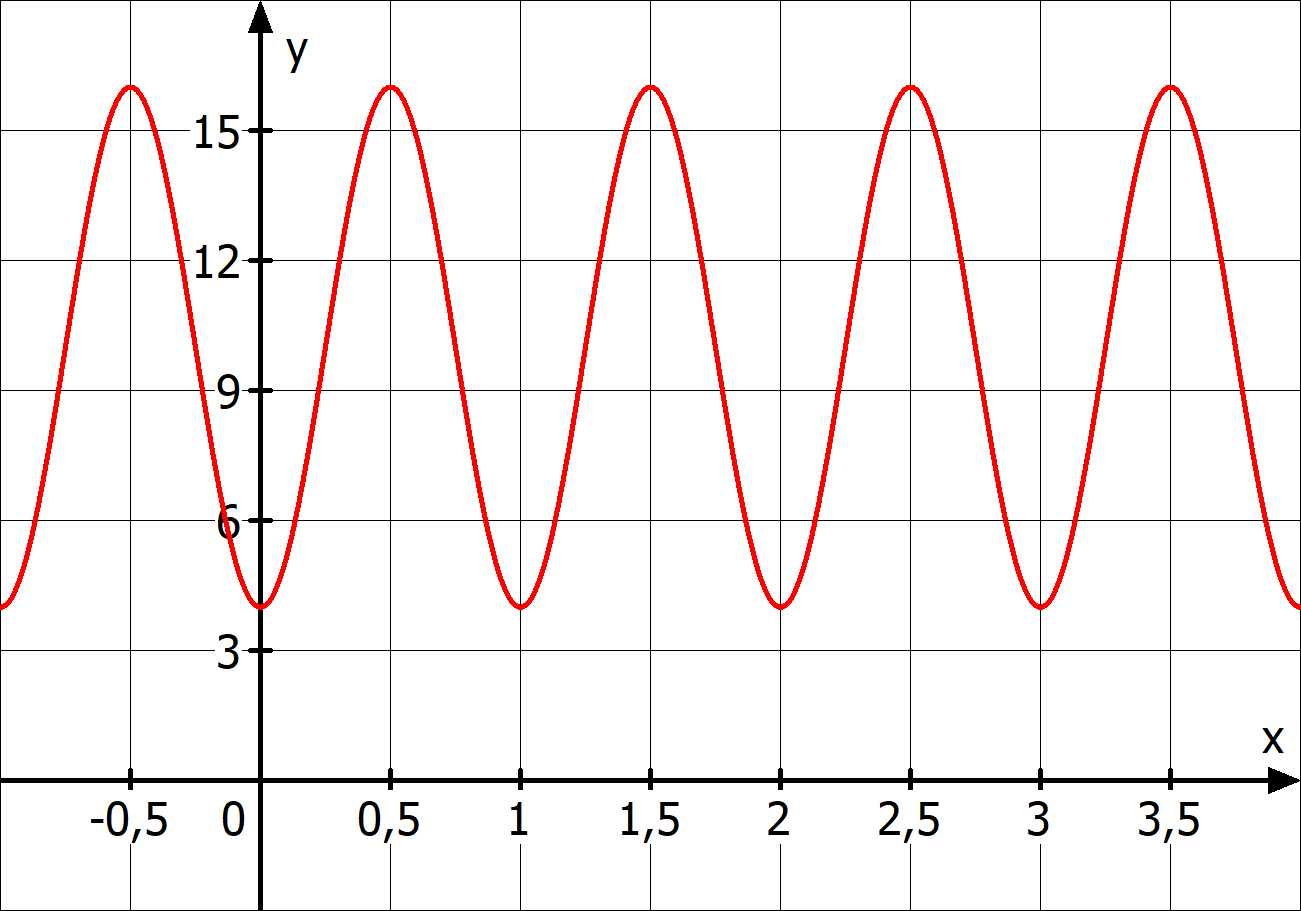
\includegraphics[height=5cm]{\trigonometrie/pics/AllgSinA1_20.png}
	\end{enumerate}
\end{Answer}
\begin{Answer}[ref=allgSinCosA2]
	\begin{enumerate}[label=\alph*)]
		\item \(f_1(x)=2\sin\left(x\right)+1\)
		\item \(f_2(x)=-\sin\left(\frac{1}{2}x\right)-1\)
		\item \(f_3(x)=1,5\cos\left(\pi x\right)+0,5\)
		\item \(f_4(x)=-3\cos\left(2\pi x\right)+3\)
		\item \(f_5(x)=-\cos\left(4x\right)+2\)
		\item \(f_6(x)=-0,5\sin\left(\frac{3}{2}x\right)+1\)
		\item \(f_7(x)=\sin\left(\frac{3\pi}{2}x\right)-0,5\)
		\item \(f_8(x)=-3\sin\left(4\pi x\right)-1\)
		\item \(f_9(x)=-2,5\cos\left(2\pi x\right)-5\)
		\item \(f_{10}(x)=\sin\left(\frac{1}{4} x\right)-0,75\)
	\end{enumerate}
\end{Answer}